\documentclass[12pt]{article}
\usepackage{fullpage}
\usepackage[normalem]{ulem}
\usepackage{fancyhdr,graphicx,amsmath,amssymb, mathtools, scrextend, titlesec, enumitem}
\usepackage[ruled,vlined]{algorithm2e} 
\usepackage{listings}
\usepackage{mathtools}
\usepackage{subcaption}
\usepackage{float}
\usepackage{bm}
\DeclarePairedDelimiter{\norm}{\lVert}{\rVert}
\DeclarePairedDelimiter{\abs}{\lvert}{\rvert}

\title{4M17 Coursework \#2: Practical Optimisation}
\author{CCN: \textbf{5673D}}
\begin{document}
\maketitle

\begin{enumerate}
	\item \textbf{Simulated Annealing}
	\begin{enumerate}
	\item \textbf{Problem-Specific Implementation Details}
	\begin{itemize}
		\item The specific implementation of simulated annealing used for this problem followed many of the suggestions in the 4M17 Simulated Annealing notes and was coded by myself in Python3. The full source code, along with comments, can be found in the Appendix. With regards to specific details, in some cases in the notes there were multiple suggestions as to best practice. With this in mind, I've implemented a few methods (and will evaluate them in more detail in a future section).
		\item \textbf{Burn-In}: I implemented a 'burn-in' period where I randomly sampled the function for a few iterations. I chose my start point $x_{\text{init}}$ to be the best random $x$ that resulted in the lowest objective function evaluation. 
		\item Moreover, I also used these results to form the basis of my \textbf{Initial Temperature}. I explored both using the standard deviation of objective function differences and also setting the temperature such that the probability of accepting an increase in objective function increase was $\bm{P}_{\text{init}}$.
		\item \textbf{Solution Generation}: New solutions were generated using the method suggested by Parks (1990) and the control variables $x$ were scaled to be in the range of (-1, 1). Alternative methods such as using the constant diagonal matrix $\bm{C}$ were also implemented. However, the method by Vanderbilt (1984) was not implemented owing to the need to use Cholesky decomposition, as well as the additional difficulty of calculating $\bm{X}$.
		\item \textbf{Constraints}: The nature of the task defined limits on the control variables such that $abs(x_{i}) \leq 512$ for every dimension. These constraints were handled by clipping values of $\bm{x}$ that left the bounded region. I also investigated with an alternative mechanism where I would ignore any generated point outside the problem bounds and would instead re-generate the control variable. This method didn't yield as strong a result (across both the 2D and 5D case - irrespective of the algorithm used).
		\item \textbf{Solution Assessment}: The probability of accepting a solution is as in the notes. Two different methods were used to calculate $p$ - depending on the nature of the process used for Solution Generation (i.e. when using Parks' method, there is an additional $\bar{d}$ term on the denominator in the exponent).
		\item \textbf{Temperature Decrement}: Temperatures were decremented in two ways: either with the simple exponential cooling scheme or with the adaptive annealing schedule proposed by Huang (1996).
		\item \textbf{Final Temperature}: The search is halted with the enhanced method in the notes: when there is no improvement in the global solution over the entire Markov Chain and the acceptance ratio falls below a threshold value $\bm{\chi_{f}}$). A hard cut=off was also placed when 10000 objective function evaluations had occurred, as specified by the task. 
		\item \textbf{Other}: Restarts were also implemented although there was no need for them in the 2D Eggholder case. Finally, \textbf{Markov Chain lengths} $L_{k}$ were chosen such that there could be a large number of chains within the 10000 objective function evaluation limits.
	\end{itemize}
	\item \textbf{Evaluation on 2D Eggholder Function}
	\begin{itemize}
		\item To demonstrate that Simulated Annealing is working, I ran my vanilla implementation on the 2D Eggholder function and, after 50 runs, the minimum objective function was determined to be $-959.6406600$ at $[512, 404.23025855]$. In every case, the algorithm terminates far before performing 10000 objective function evaluations (the maximum allowable limit).
		\item This value is very close (within $< 0.001\%$ error) to the true global minima in this region (listed online as $−959.6406627$).
		\item In addition, it's also necessary to show that the walks that Simulated Annealing go through at a given temperature are also reasonable. With this in mind, it is clear from Figure \ref{fig1} that the algorithms' walks are sensible; Initially, when the temperature is high, the walk traverses the entire state-space in a seemingly random manner (which makes sense as all updates will be accepted)
		\item However, as the temperature lowers, the walks become less random/dense and begin to converge to a localised area. At the lowest temperature, the walk traverses only  around the local minimum as in Figure \ref{fig1}d. In this case, the local minimum is in fact global minimum although this isn't necessarily always the case. 
		\item In the case of the 2D Eggholder, the algorithm overwhelmingly terminates at the global minimum.
		\item Another way of evaluating the algorithm is through determining the distribution of minima the algorithm terminates at. This was achieved by running the algorithm through multiple runs (i.e. 100) and binning minima into square regions of length 10. 
		\item Figure \ref{fig2} shows the histogram for these regions: with the most probable top two regions being in the immediate area around the true global minimum with a similar mean objective function value (note the $x_{2}$ values is $404$ and this will be split between the $400$ and $410$ bins. 
		\item The slight discrepancy between the 'global minimum' mean f(x) values and that of the true global minimum is likely because the algorithm likely terminates close to but not necessarily at the global minimum from run-to-run.
		\item Finally Figure \ref{fig4} shows the typical change in the objective function with the \# of iterations. The trend is generally decreasing: albeit with a lot of noise due to an initial high probability of acceptance as well as Markov Chain resets. This indicates that the SA algorithm is working well and Figure \ref{fig3} aptly shows that the algorithm does explore the state-space properly.
		\begin{figure}[ht]
		\centering
		\begin{subfigure}{8cm}
		\centering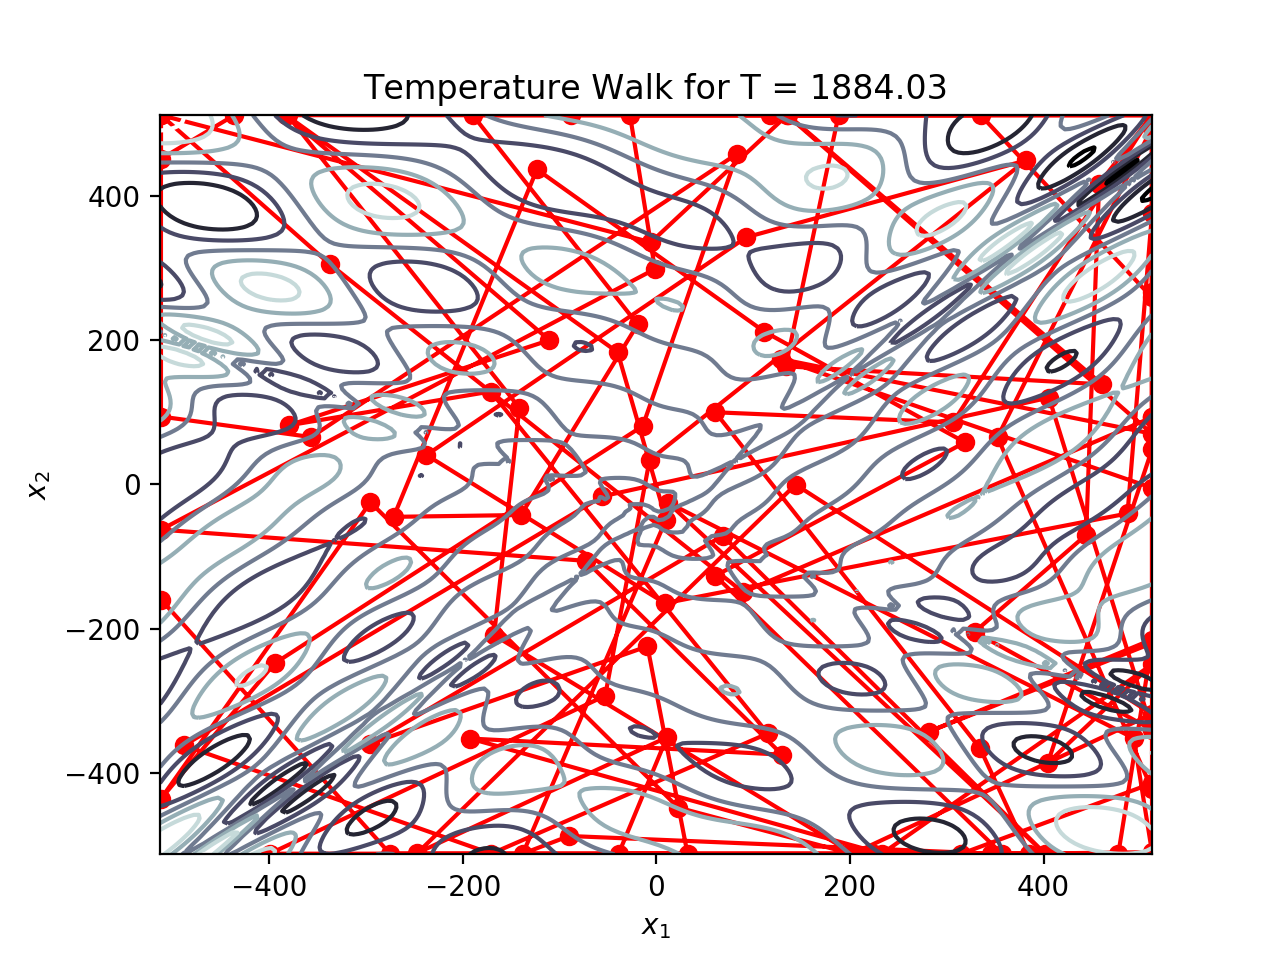
\includegraphics[width=8cm]{a_T_1}
		\caption{Temperature: 1884.03}
		\end{subfigure}%
		\begin{subfigure}{8cm}
		\centering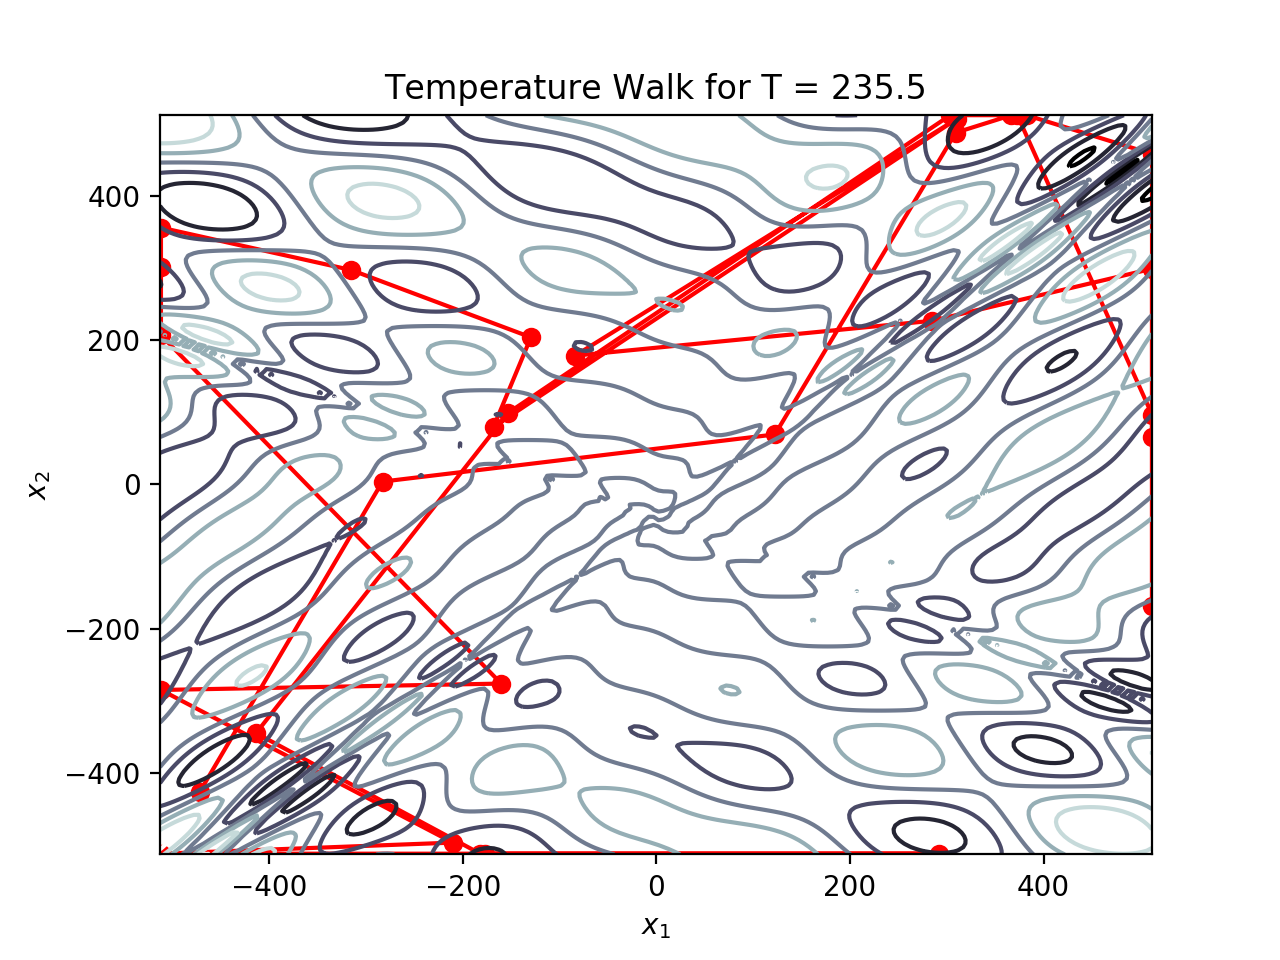
\includegraphics[width=8cm]{a_T_2}
		\caption{Temperature: 235.5}
		\end{subfigure}\vspace{10pt}
		\begin{subfigure}{8cm}
		\centering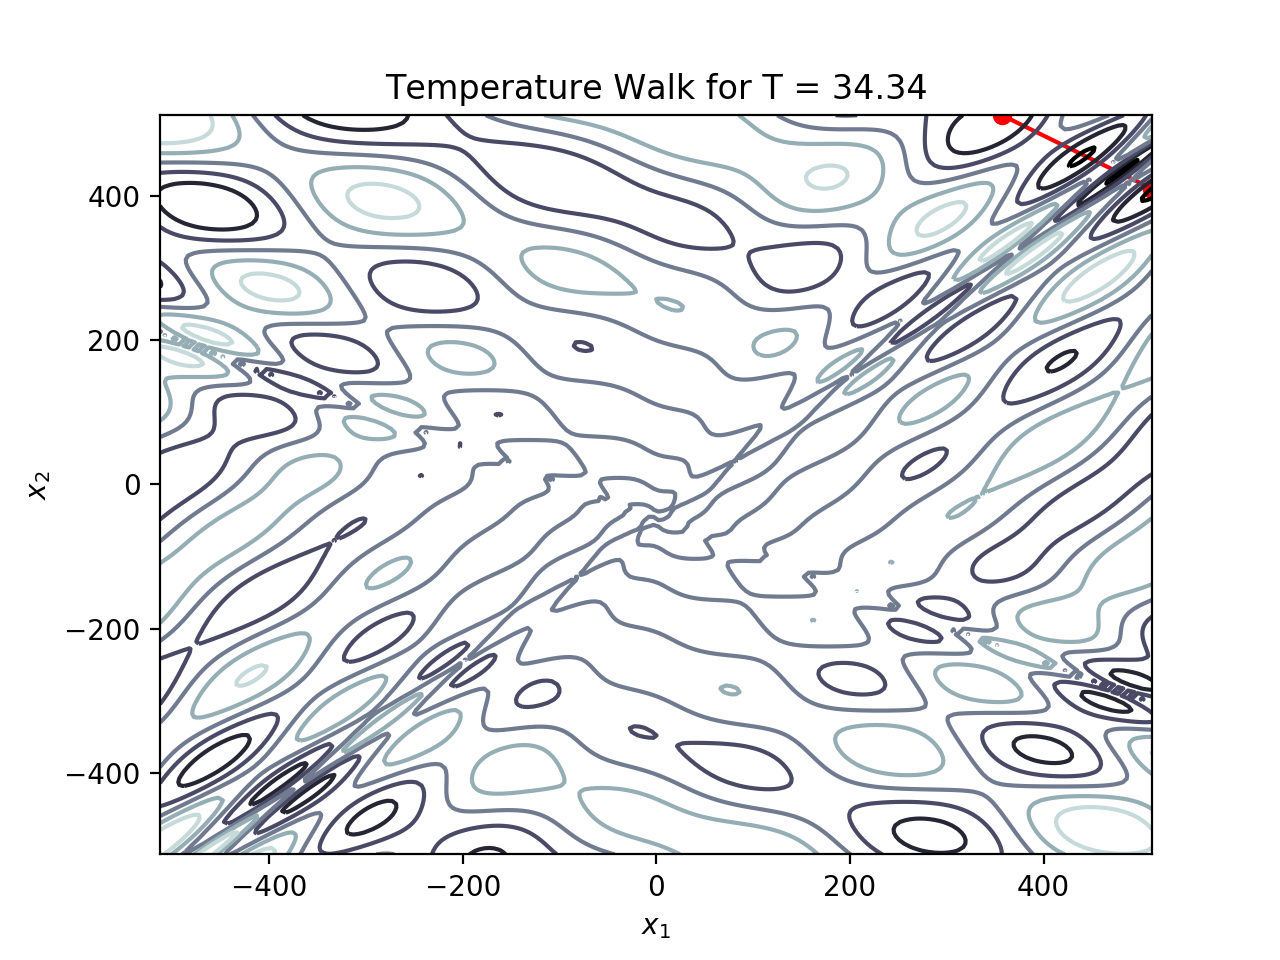
\includegraphics[width=8cm]{a_T_3}
		\caption{Temperature: 34.34}
		\end{subfigure}%
		\begin{subfigure}{8cm}
		\centering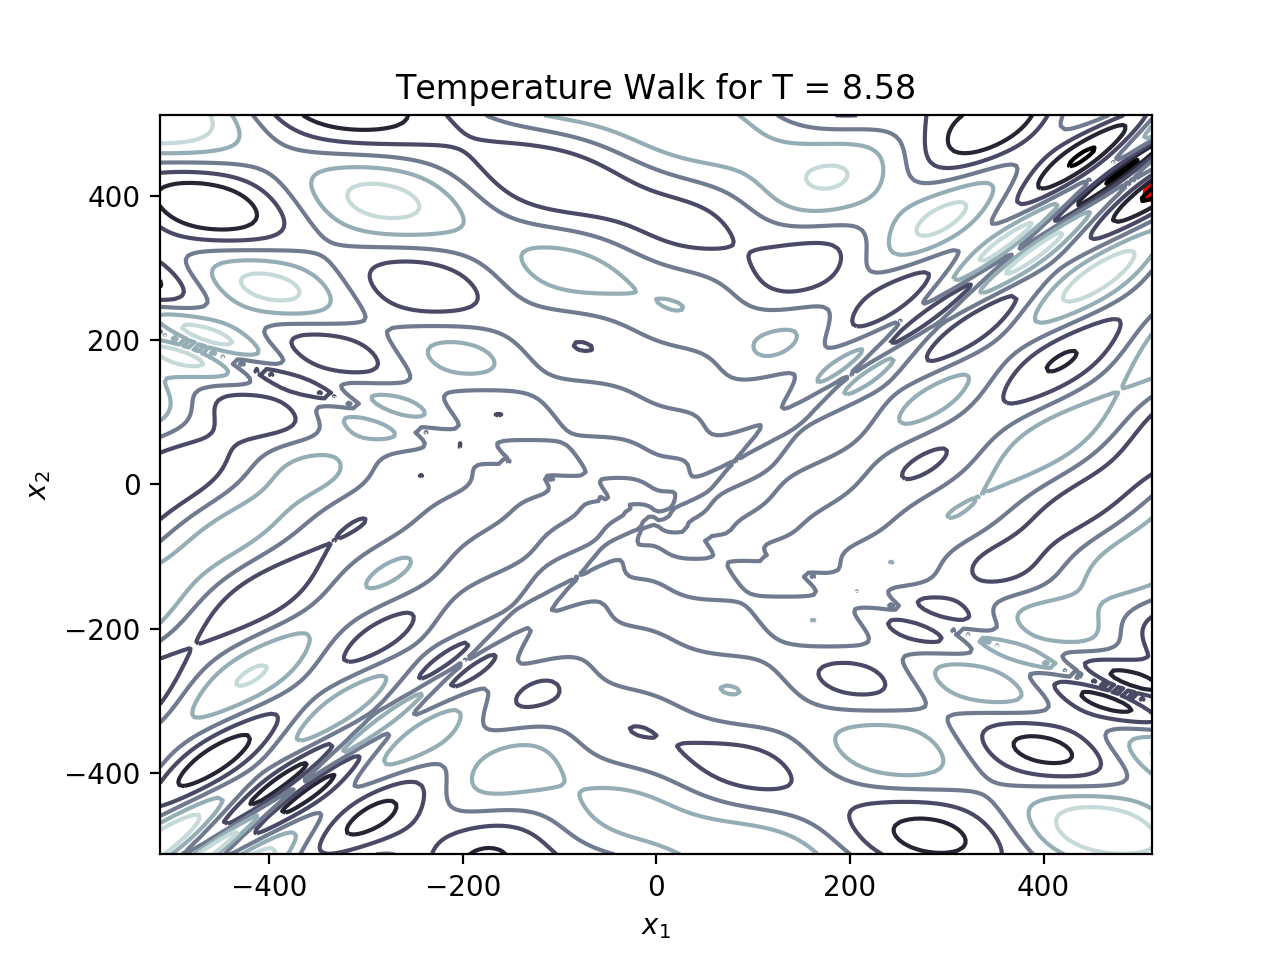
\includegraphics[width=8cm]{a_T_4}
		\caption{Temperature: 8.58}
		\end{subfigure}
		\caption{Simulated Annealing walk at different temperatures}
		\label{fig1}
		\end{figure}
		\begin{figure}[H]
		\centering
		\begin{subfigure}{8cm}
		\centering
		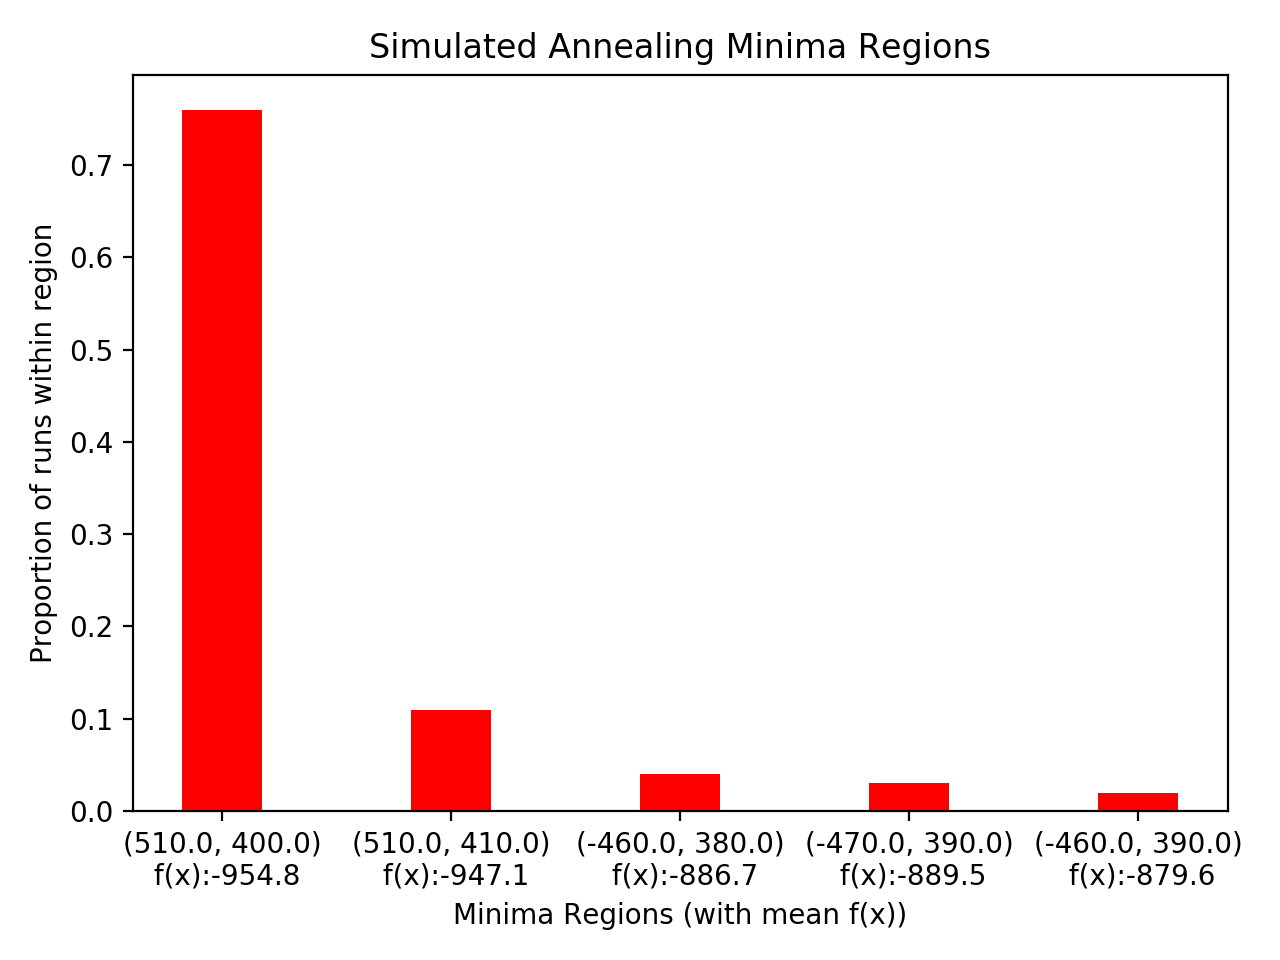
\includegraphics[width=8cm]{a_hist_bin}
		\caption{Histogram Regions}
		\end{subfigure}%
		\begin{subfigure}{8cm}
		\centering
		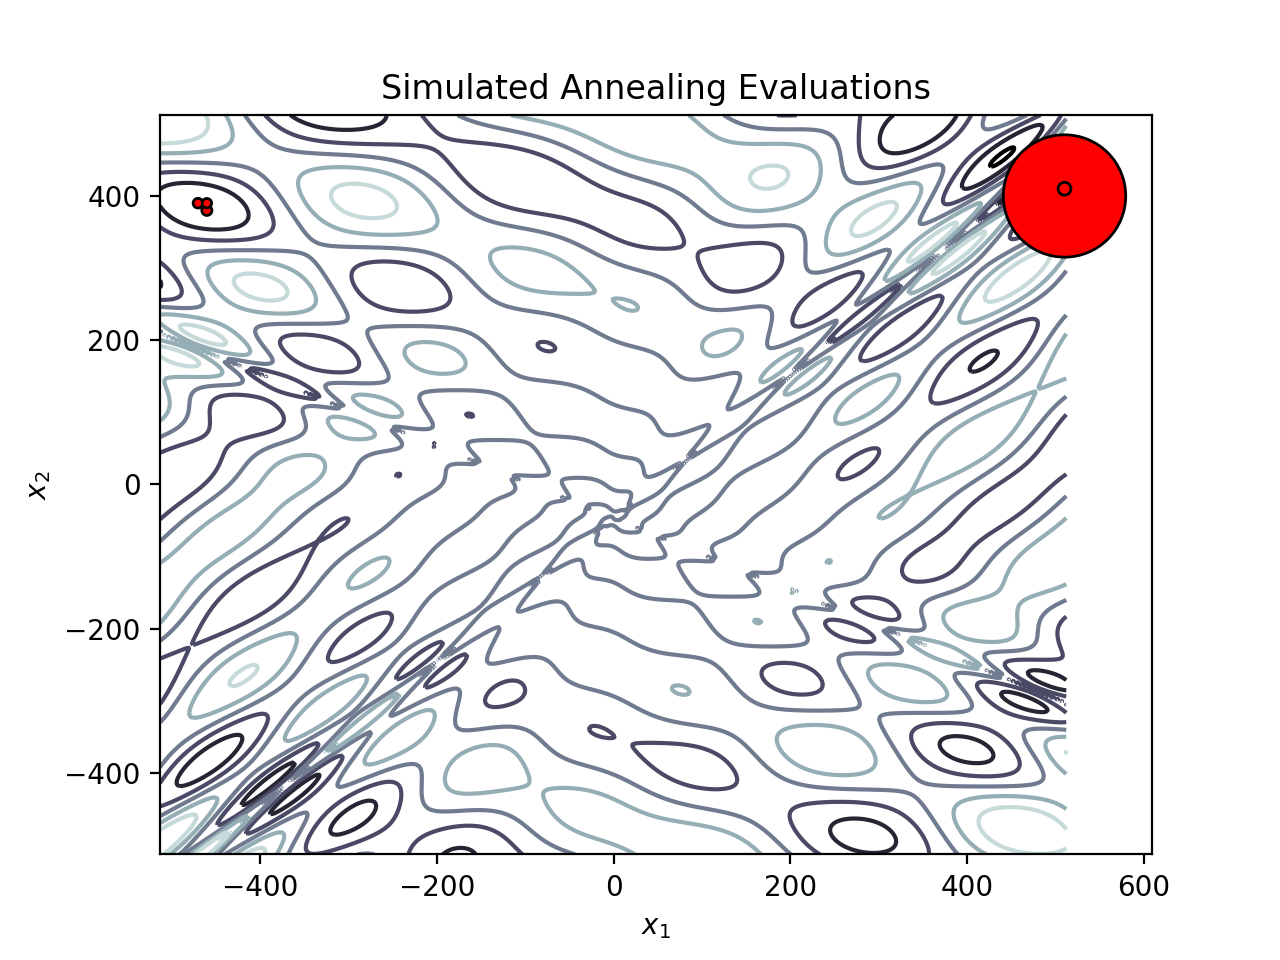
\includegraphics[width=8cm]{a_hist_plot}
		\caption{Regions on plot (with relative frequency)}
		\end{subfigure}
		\caption{Minima regions found after 100 iterations. Global minimum at $[512, 404]$}
		\label{fig2}
		\end{figure}
		\begin{figure}[H]
		\centering
		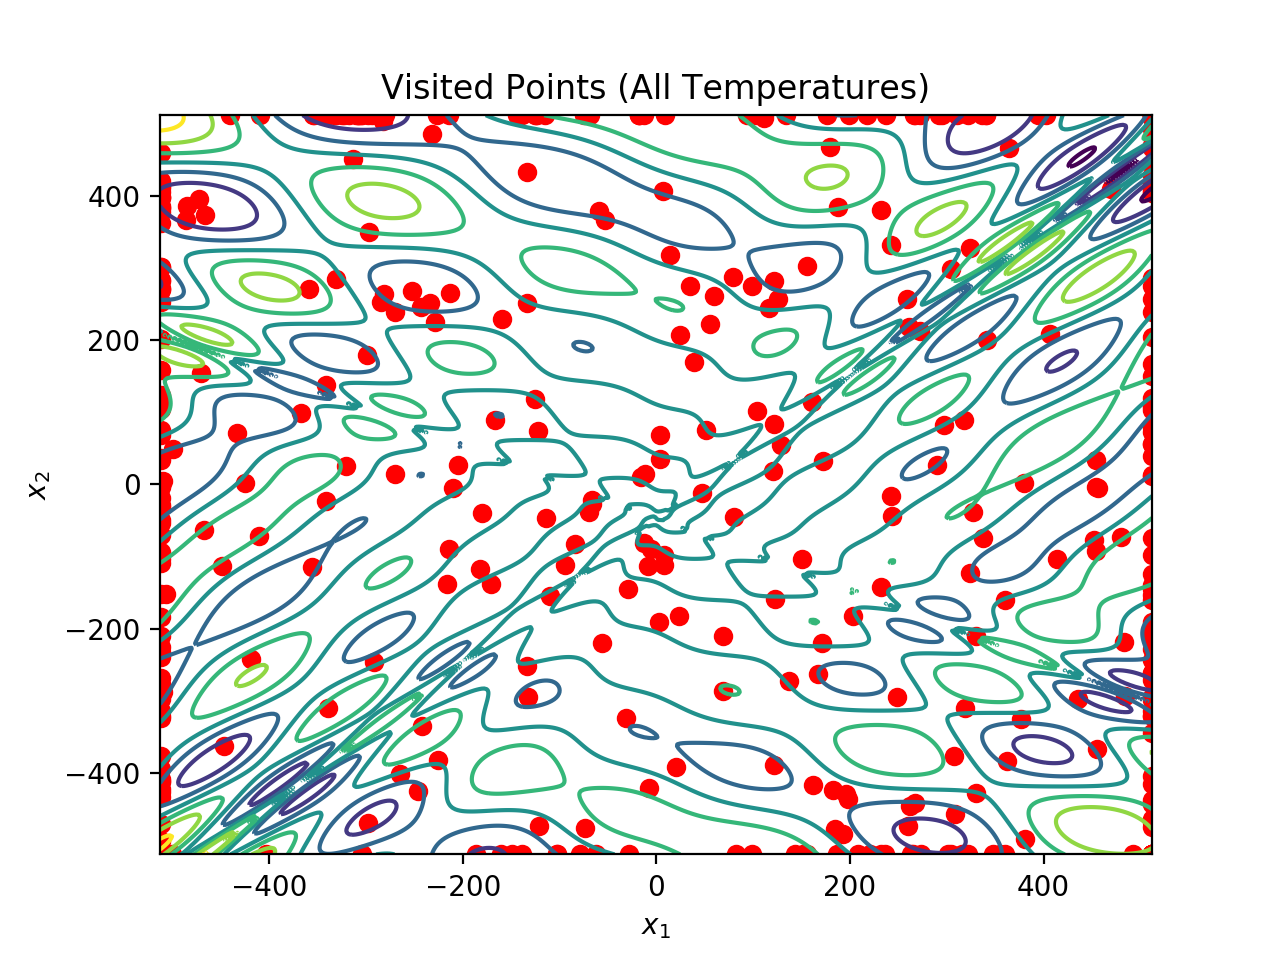
\includegraphics[width=\textwidth]{a_search_typical.png}
		\caption{A typical search pattern of a Simulated Annealing run}
		\label{fig3}
		\end{figure}
		\begin{figure}[H]
		\centering
		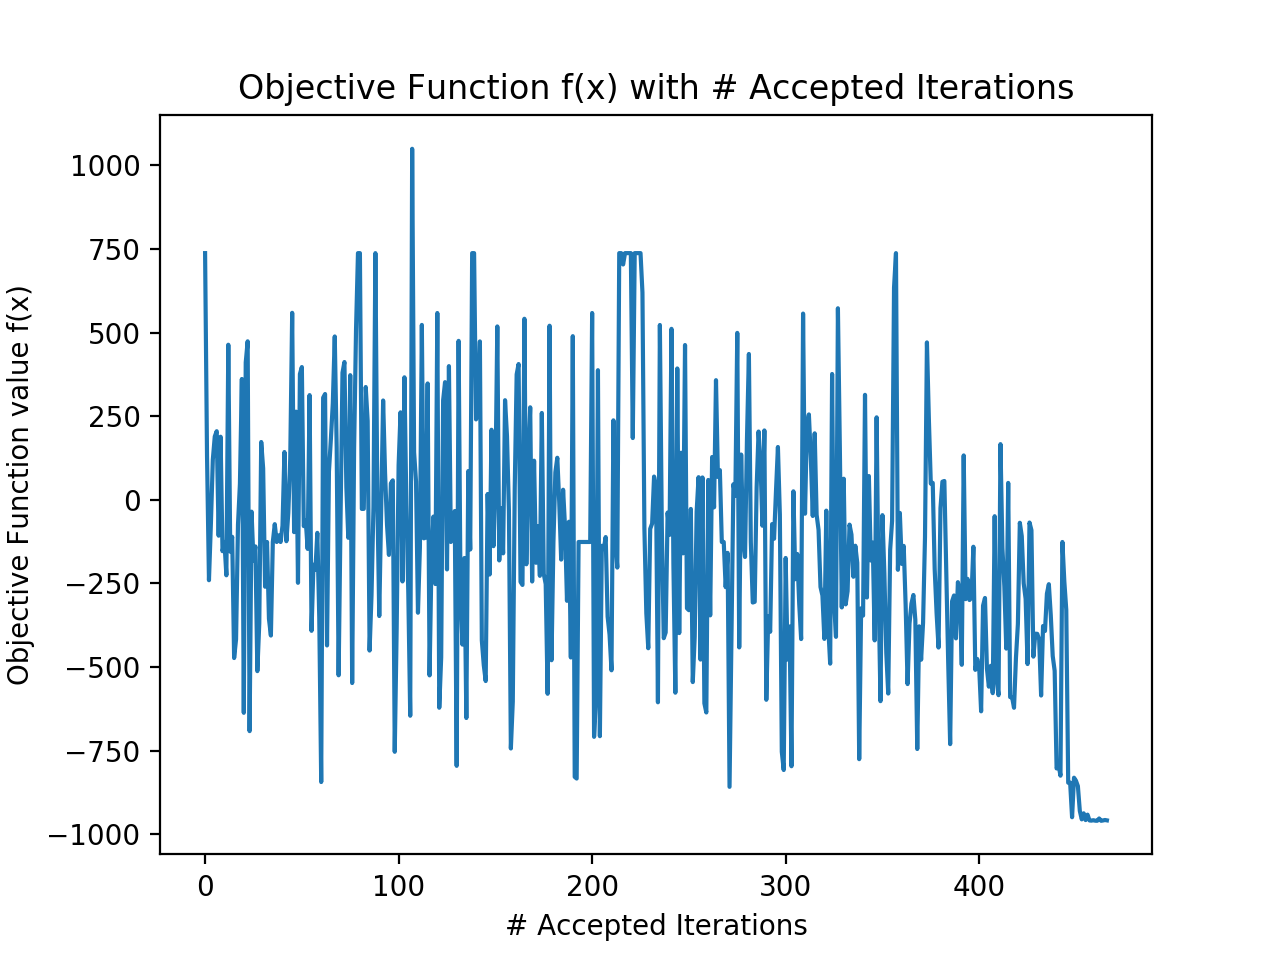
\includegraphics[width=\textwidth]{a_f_plot}
		\caption{A typical variation in objective function with \# accepted iterations}
		\label{fig4}
		\end{figure}

	\end{itemize}
	\item \textbf{Evaluation on 3D Egghodler Function}
	\end{enumerate}
\end{enumerate}
\end{document}